
\begin{frame}{A generic update engine for dynamic pivoting}
\framesubtitle{Update Issue}
\begin{columns}
\begin{column}{.50\textwidth}
\begin{center}
\includegraphics[scale=0.5]{update_swap.png}
\end{center}
\end{column}
\hfill
\begin{column}{.50\textwidth}
The main tile exchange swap rows with other concerned tile.
\pause
\begin{exampleblock}{Problem}
\begin{itemize}
\item A dynamic decision for a static DAG \\
\pause
$\Longrightarrow$ Prepare tasks for all possible communications?
\end{itemize}
\end{exampleblock}{}
\end{column}
\end{columns}
\end{frame}

\begin{frame}{A generic update engine for dynamic pivoting}
\framesubtitle{Solutions}
Ideas:
\begin{itemize}
\item Avoiding useless swap\\
\pause
$\rightarrow$ Use of permutations instead of pivots index
\pause
\item Updating the main tile is more urgent\\
\pause
$\rightarrow$ Parallelize the swap \textbf{from} and the swap \textbf{into} the main tile with a priority for the second
\pause
\item Minimizing the number of communication (not the volume)\\
\pause
$\rightarrow$ Gather communications of all rows over two buffer
\end{itemize}
\pause
\begin{exampleblock}{}
$\rightarrow$ Five kind of tasks : COPY, COLLECT, RECEIVE, SEND and PASTE.
\end{exampleblock}{}

\end{frame}

\begin{frame}{A generic update engine for dynamic pivoting}
\framesubtitle{Task Flow of Update}
Exemple of the update tasks dependacies for a panel of 16 tiles over 4 nodes :
\begin{center}
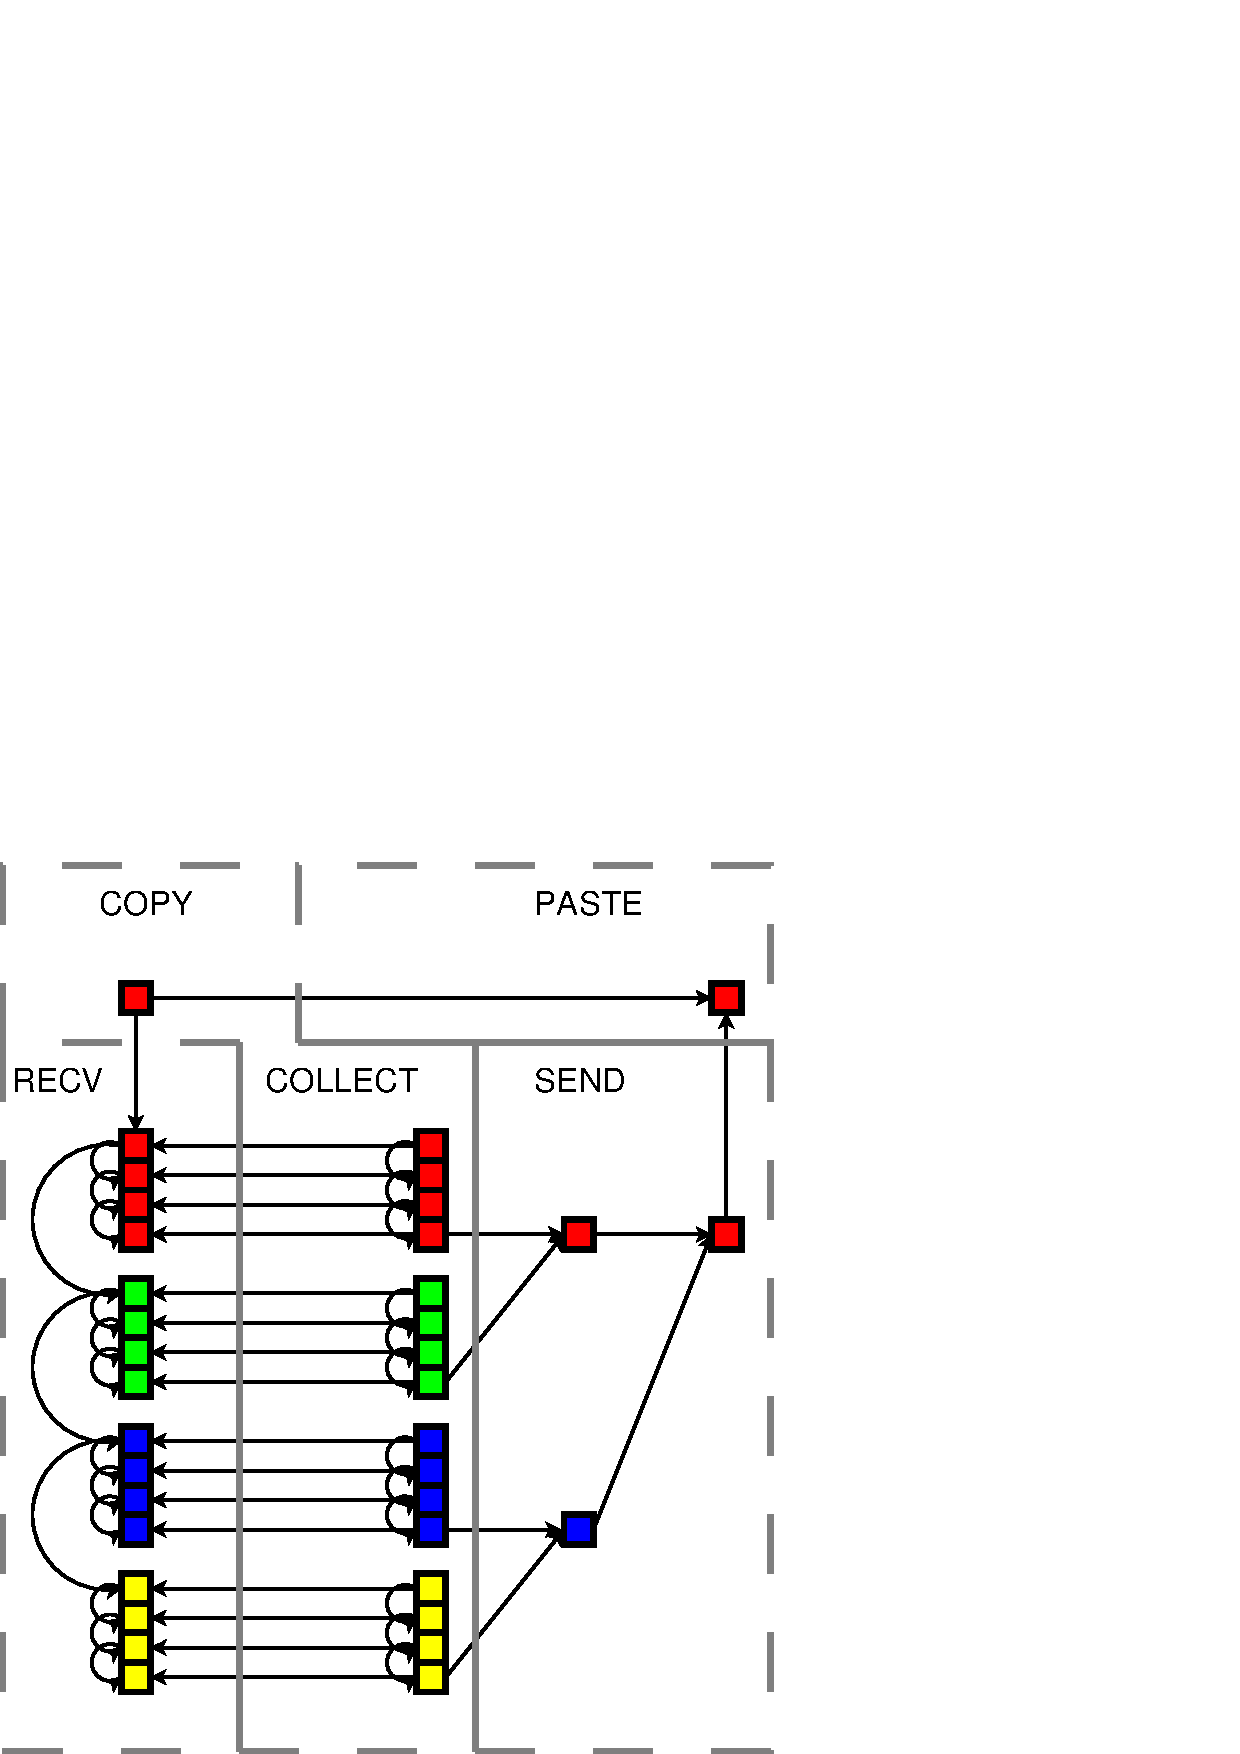
\includegraphics[scale=0.5]{swap_opt.png}
\end{center}
\end{frame}

\begin{frame}{A generic update engine for dynamic pivoting}
\framesubtitle{Update Impact}
\begin{center}
\includegraphics[width=0.7\textwidth]{dgetrf_update_problem.png} 
\end{center}
\end{frame}

\begin{frame}{A generic update engine for dynamic pivoting}
\framesubtitle{Results}
\begin{itemize}
\item Small impact on the performance
\item A generic update engine
\end{itemize}
\end{frame}